\documentclass{article}
\usepackage{tikz}
\usepackage{amsmath, amssymb, amsthm}
% Customization ---------------

% GEOMETERY
% sets paper size, margins and a parameter 
\usepackage[letterpaper, top=1.3in, bottom=1.3in, left=1.3in, right=1.3in,heightrounded]{geometry}

%Background
\usepackage{background}
\backgroundsetup{
 scale=1,
 color=black,
 opacity=10,
 angle=0,
 contents={
  \includegraphics[width=\paperwidth,height=\paperheight]{brand.pdf}
 }
}
%Line Height 
\renewcommand{\baselinestretch}{1.25} %Line spacing

%Par Skip and parindent
\setlength{\parindent}{0pt}
\setlength{\parskip} {1.2em}
\usetikzlibrary{arrows}

\newcommand{\vect}[1]{\langle #1 \rangle}
\begin{document}


\title{\bf CSCI 340, Winter 2025\\ Math HW02}
\author{\textbf{Name}: \textit{Abid Jeem}}
\date{\today}

\maketitle

\begin{enumerate}

\item
  In the picture below, $a$, $b$, and $c$ are arbitrary points, and
  the dotted line from $b$ to $x$ is perpendicular to the line from
  $a$ to $c$. Give formulas to find each of the
  distances from 
  $a$, $b$, and $c$ to $x$ as a function of the points $a$, $b$, and $c$.
  Use point subtraction and dot products. Each formula should stand
  on its own and not depend on the other formulas.

\newcommand{\mypoint}[3] {
  \node (#1) at (#2) {};
  \fill (#2) circle (2pt);
  \node[anchor=#3] (label#1) at (#2) {$#1$};
  }
\begin{tikzpicture}
%  \draw[help lines] (0,0) grid (8,5);
  \mypoint{a}{1,3}{east};
  \mypoint{b}{5,5}{south};
  \mypoint{c}{8,1}{west};
  \mypoint{x}{4.2,2.1}{north};
\draw (a) -- (b) -- (c) -- (a);
\draw[dotted] (b) -- (x);
\end{tikzpicture}

 \bigskip
  
 \section*{Solution}

Here, \(x\) is the orthogonal projection of \(b\) onto the line passing through \(a\) and \(c\). Parameterizing the line, we get any point:

\begin{equation}
x = a + \lambda (c - a)
\label{eq:x_param}
\end{equation}


Applying the dot product condition for orthogonal vectors, we get:

\[
(x - b) \cdot (c - a) = 0
\]

\vspace{0.5cm}

Substituting \(x = a + \lambda (c - a)\),

\[
(a + \lambda (c - a) - b) \cdot (c - a) = 0
\]

\[
=> (a - b + \lambda (c - a)) \cdot (c - a) = 0
\]

\[
=> (a - b) \cdot (c - a) + \lambda (c - a) \cdot (c - a) = 0
\]

Solving for \(\lambda\),

\[
\lambda = \frac{(b - a) \cdot (c - a)}{(c - a) \cdot (c - a)}
\]

Placing \(\lambda\) in equation (1), we get—

\begin{equation}
x = a + \frac{(b - a) \cdot (c - a)}{(c - a) \cdot (c - a)} (c - a)
\label{eq:x_projection}
\end{equation}


\subsection*{Distance from \(a\) to \(x\)}

Equation (2) - \(a\):

\[
x - a = \frac{(b - a) \cdot (c - a)}{(c - a) \cdot (c - a)} (c - a)
\]

Taking its Euclidean norm,

\[
\boxed{\|x - a\| = \left|\frac{(b - a) \cdot (c - a)}{(c - a) \cdot (c - a)}\right| \|c - a\|}
\]

\subsection*{Distance from \(c\) to \(x\)}

\(c\) - Equation (2):

\[
c - x = c - \left(a + \frac{(b - a) \cdot (c - a)}{(c - a) \cdot (c - a)} (c - a) \right)
\]

\[
=> c - x = \left(1 - \frac{(b - a) \cdot (c - a)}{(c - a) \cdot (c - a)} \right) (c - a)
\]

Taking its Euclidean norm,

\[
\boxed{\|c - x\| = \left|1 - \frac{(b - a) \cdot (c - a)}{(c - a) \cdot (c - a)}\right| \|c - a\|}
\]

\subsection*{Distance from \(b\) to \(x\)}

Equation (2) - \(b\):

\[
x - b = (a - b) + \frac{(b - a) \cdot (c - a)}{(c - a) \cdot (c - a)} (c - a)
\]

Taking its Euclidean norm,

\[
\boxed{\|x - b\| = \left\|(b - a) - \frac{(b - a) \cdot (c - a)}{(c - a) \cdot (c - a)}\, (c - a)\right\|}
\]



  \newpage
  
\item Suppose we specify a camera by five points: the eye position and the four corners of
  the image plane (upper left, upper right, lower left, lower right),
  as in the figure below (the left side of the view plane is deeper
  into the picture than the right side). 

    \tikzset{>=latex}
    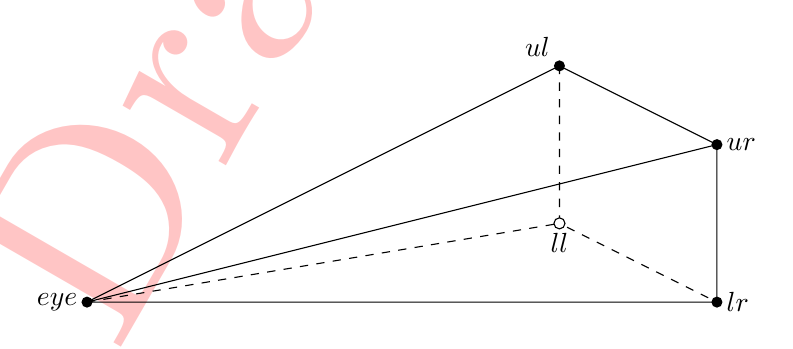
\begin{tikzpicture}

      \draw (1,2) -- (7,5) -- (9,4) -- (9,2) -- cycle;
      \draw (1,2) -- (9,4);
      \draw [dashed] (1,2) -- (7,3);
      \draw [dashed] (7,5) -- (7,3) -- (9,2);
      
      \fill (1,2) circle (2pt) node[anchor=east] {$eye$};
      \fill (7,5) circle (2pt) node[anchor=south east] {$ul$};
      \fill (9,4) circle (2pt) node[anchor=west] {$ur$};
      \fill (9,2) circle (2pt) node[anchor=west] {$lr$};      
      \draw[fill=white] (7,3) circle (2pt) node[anchor=north] {$ll$};
      
    \end{tikzpicture}

Given a position in the image plane defined by $percentX$ and $percentY$ (in percent coordinates), 
and with the origin of the image plane understood
as the upper left corner, write an expression giving the vector for a
ray from the eye to that point in the view plane. You do not need to
normalize the vector.

\section*{Solution}

Here, 
\[
World_{\text{top}} = ul + \; percentX \,(ur - ul)
\]

\[
World_{\text{bottom}} = ll + \; percentX \,(lr - ll)
\]

\[
WorldCoordinate = World_{\text{top}} + \; percentY \,(World_{\text{bottom}} - World_{\text{top}})
\]

\medskip

Therefore, 
\[
\text{ray} = WorldCoordinate - eye
\]

Thus, 
\[
\boxed{\text{ray} = (World_{\text{top}} + \; percentY \,(World_{\text{bottom}} - World_{\text{top}})) - eye}
\]

\newpage

\item Given a camera specified as in the lecture notes, with an eye
  position, normalized right, up, and foward vectors, and scalars depth,
  width and height, $\langle p, r, u, f, d, w, h\rangle$, write
  expressions for each of the four corner points in the camera representation
  from the previous problem and the center/focus.
  \section*{Solution}
\begin{align*}
(a) \quad c &= p + d f \\
(b) \quad ul &= c + \frac{h}{2} u- \frac{w}{2} r  \\
(c) \quad ur &= c + \frac{h}{2} u+ \frac{w}{2} r  \\
(d) \quad ll &= c - \frac{h}{2} u - \frac{w}{2} r \\
(e) \quad lr &= c - \frac{h}{2} u+ \frac{w}{2} r 
\end{align*}

  
\newpage

\item For each of the following implicitly defined quadric surfaces,
  find fomulas for  the coefficients  for the quadratic equation,
  $at^2 + bt + c = 0$
  to determine the value of $t$ where a ray defined by $p + tv$
  intersects the surface. 
    
    \section*{Solution}
    Given Elliptic Paraboloid,
    
    \[\frac{x^2}{a^2} + \frac{y^2}{b^2} - z\ = 0\]
\vspace{0.5cm}

    Points on the line generated by:
    \[
    p + t v = (p_x, p_y, p_z) + t (v_x, v_y, v_z)
    \]
    Pluggin it in:

    \[
    \frac{(p_x + t v_x)^2}{a^2} + \frac{(p_y + t v_y)^2}{b^2} - (p_z + t v_z) = 0
    \]

    \[
    \Rightarrow \frac{p_x^2 + 2t p_x v_x + t^2 v_x^2}{a^2} + \frac{p_y^2 + 2t p_y v_y + t^2 v_y^2}{b^2} - (p_z + t v_z) = 0
    \]

    \[
    \Rightarrow \left( \frac{v_x^2}{a^2} + \frac{v_y^2}{b^2} \right)t^2 + \left( \frac{2 p_x v_x}{a^2} + \frac{2 p_y v_y}{b^2} - v_z \right)t + \left( \frac{p_x^2}{a^2} + \frac{p_y^2}{b^2} - p_z \right) = 0
    \]

    Therefore,

    \[
\boxed{
\begin{aligned}
a &= \frac{v_x^2}{a^2} + \frac{v_y^2}{b^2}\\[1mm]
b &= \frac{2\,p_x\,v_x}{a^2} + \frac{2\,p_y\,v_y}{b^2} - v_z\\[1mm]
c &= \frac{p_x^2}{a^2} + \frac{p_y^2}{b^2} - p_z
\end{aligned}
}
\]
\vspace{1cm}

\section*{Solution}

  Given the hyperbolic paraboloid equation,

\[
\frac{x^2}{a^2} - \frac{y^2}{b^2} - z = 0
\]

Points on the line generated by:

\[
p + t v = (p_x, p_y, p_z) + t (v_x, v_y, v_z)
\]

Plugging it in:

\[
\frac{(p_x + t v_x)^2}{a^2} - \frac{(p_y + t v_y)^2}{b^2} - (p_z + t v_z) = 0
\]

\[
\Rightarrow \frac{p_x^2 + 2t p_x v_x + t^2 v_x^2}{a^2} - \frac{p_y^2 + 2t p_y v_y + t^2 v_y^2}{b^2} - (p_z + t v_z) = 0
\]

\[
\Rightarrow \left( \frac{v_x^2}{a^2} - \frac{v_y^2}{b^2} \right)t^2 + \left( \frac{2 p_x v_x}{a^2} - \frac{2 p_y v_y}{b^2} - v_z \right)t + \left( \frac{p_x^2}{a^2} - \frac{p_y^2}{b^2} - p_z \right) = 0
\]

Therefore,

\[
\boxed{
\begin{aligned}
a &= \frac{v_x^2}{a^2} - \frac{v_y^2}{b^2}\\[1mm]
b &= \frac{2\,p_x\,v_x}{a^2} - \frac{2\,p_y\,v_y}{b^2} - v_z\\[1mm]
c &= \frac{p_x^2}{a^2} - \frac{p_y^2}{b^2} - p_z
\end{aligned}
}
\]
\vspace{4cm}

    \section*{Solution}
Elliptic hyperboloid of one sheet, \[\frac{x^2}{a^2} + \frac{y^2}{b^2} - \frac{z^2}{c^2}\ = 1\]
  \[
\Rightarrow\frac{(p_x + t\,v_x)^2}{a^2} + \frac{(p_y + t\,v_y)^2}{b^2} - \frac{(p_z + t\,v_z)^2}{c^2} = 1
\]
\[
\Rightarrow \left( \frac{v_x^2}{a^2} + \frac{v_y^2}{b^2} - \frac{v_z^2}{c^2} \right)t^2 + \left( \frac{2 p_x v_x}{a^2} + \frac{2 p_y v_y}{b^2} - \frac{2 p_z v_z}{c^2} \right)t + \left( \frac{p_x^2}{a^2} + \frac{p_y^2}{b^2} - \frac{p_z^2}{c^2} - 1 \right) = 0
\]

Therefore,

\[
\boxed{
\begin{aligned}
a &= \frac{v_x^2}{a^2} + \frac{v_y^2}{b^2} - \frac{v_z^2}{c^2}\\[1mm]
b &= \frac{2\,p_x\,v_x}{a^2} + \frac{2\,p_y\,v_y}{b^2} - \frac{2\,p_z\,v_z}{c^2}\\[1mm]
c &= \frac{p_x^2}{a^2} + \frac{p_y^2}{b^2} - \frac{p_z^2}{c^2} - 1
\end{aligned}
}
\]
\newpage
\section*{Solution}

Elliptic hyperboloid of two sheets,
    \[ \frac{x^2}{a^2} + \frac{y^2}{b^2} - \frac{z^2}{c^2} = -1\]

    \[
\Rightarrow\frac{(p_x + t\,v_x)^2}{a^2} + \frac{(p_y + t\,v_y)^2}{b^2} - \frac{(p_z + t\,v_z)^2}{c^2} = -1
\]
\[
\Rightarrow \left( \frac{v_x^2}{a^2} + \frac{v_y^2}{b^2} - \frac{v_z^2}{c^2} \right)t^2 + \left( \frac{2 p_x v_x}{a^2} + \frac{2 p_y v_y}{b^2} - \frac{2 p_z v_z}{c^2} \right)t + \left( \frac{p_x^2}{a^2} + \frac{p_y^2}{b^2} - \frac{p_z^2}{c^2} + 1 \right) = 0
\]

Therefore,

\[
\boxed{
\begin{aligned}
a &= \frac{v_x^2}{a^2} + \frac{v_y^2}{b^2} - \frac{v_z^2}{c^2}\\[1mm]
b &= \frac{2\,p_x\,v_x}{a^2} + \frac{2\,p_y\,v_y}{b^2} - \frac{2\,p_z\,v_z}{c^2}\\[1mm]
c &= \frac{p_x^2}{a^2} + \frac{p_y^2}{b^2} - \frac{p_z^2}{c^2} + 1
\end{aligned}
}
\]

\newpage

Find a formula for a vector normal to each of the following
  surfaces, given a point $(x,y,z)$ on the surface.
  \section*{Solution: Normal Vectors}

For each implicitly defined surface \( f(x, y, z) = 0 \), the normal vector is given by:

\[
\nabla f = \left( \frac{\partial f}{\partial x}, \frac{\partial f}{\partial y}, \frac{\partial f}{\partial z} \right)
\]

\begin{enumerate}
    \item Elliptic Paraboloid
   \[
\boxed{\nabla f = \left(\frac{2x}{a^2},\, \frac{2y}{b^2},\, -1\right)}
\]

    \item Hyperbolic Paraboloid
    \[
\boxed{\nabla f = \left(\frac{2x}{a^2},\, -\frac{2y}{b^2},\, -1\right)}
\]

    \item Elliptic Hyperboloid of One Sheet
    \[
\boxed{\nabla f = \left(\frac{2x}{a^2},\, \frac{2y}{b^2},\, -\frac{2z}{c^2}\right)}
\]

    \item Elliptic Hyperboloid of Two Sheets
   \[
\boxed{\nabla f = \left(\frac{2x}{a^2},\, \frac{2y}{b^2},\, -\frac{2z}{c^2}\right)}
\]
\end{enumerate}

\end{enumerate}

\end{document}
